\section{}
\textit{The system shown is a two-dimensional approximation to an automobile.}
\begin{figure}[H]
    \centering
    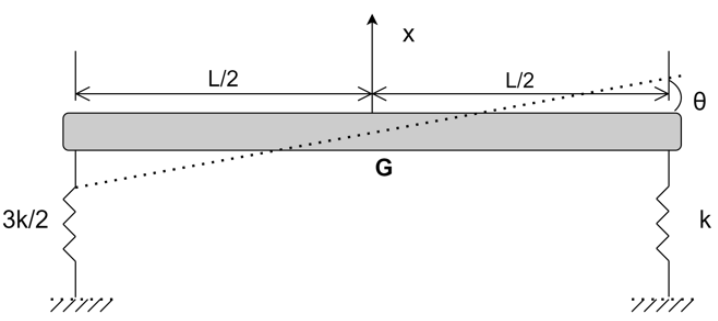
\includegraphics[width=0.5\textwidth]{Questions/Figures/Q4 Problem Diagram.png}
    \caption{Two-dimensional automobile.}
    \label{fig:Q4}
\end{figure}

\subsection{}
\textit{Using the coordinates shown determine the equations of motion.}
\begin{figure}[H]
    \centering
    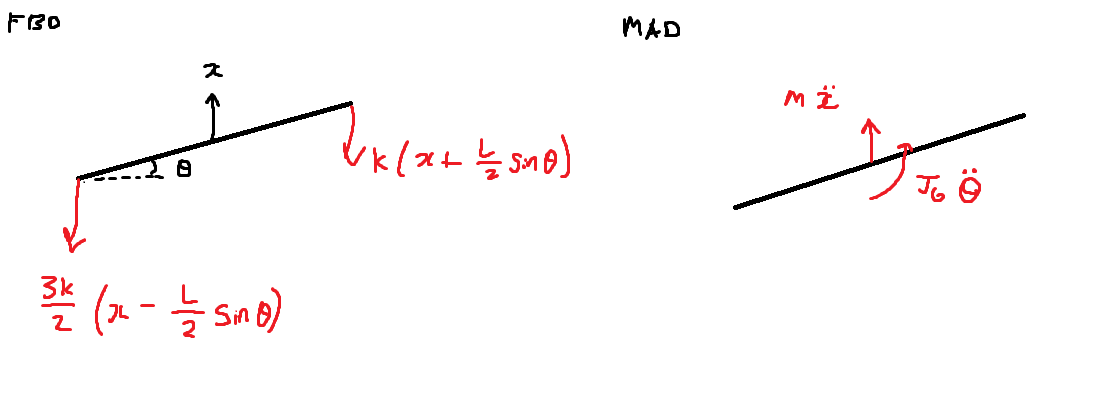
\includegraphics[width=0.5\textwidth]{Questions/Figures/Q4 FBD.png}
    \caption{Freebody diagram and mass acceleration diagram.}
    \label{fig:Q4 FBD}
\end{figure}
The freebody diagram and mass acceleration diagram is shown in Figure \ref{fig:Q4 FBD}. The equations of motion are then,
\begin{gather*}
    \uparrow \sum F_y := m \ddot{x} = -\frac{3}{2}k (x - \frac{L}{2}\theta) - k(x + \frac{L}{2}\theta) \\
    \implies m \ddot{x} + \frac{5}{2}kx - \frac{L}{4}k\theta = 0 
\end{gather*}
and, 
\begin{gather*}
    \circlearrowleft \sum M_G := J_G \ddot{\theta} = \frac{3}{2}k (x - \frac{L}{2}\theta) \frac{L}{2} - k(x + \frac{L}{2}\theta) \frac{L}{2} \\
    \implies J_G \ddot{\theta} + \frac{5}{8} kL^2 \theta - \frac{1}{4} kLx = 0
\end{gather*}
The equations of motion are then,
\begin{empheq}[box=\fbox]{align*}
    m \ddot{x} + \frac{5}{2}kx - \frac{L}{4}k\theta &= 0 \\
    J_G \ddot{\theta} + \frac{5}{8} kL^2 \theta - \frac{1}{4} kLx &= 0
\end{empheq}

\subsection{}
\textit{If $J_G = \frac{mL^2}{6}$, the equations of motion become as what follows:}
\begin{align*}
    \begin{bmatrix}
        m & 0 \\
        0 & \frac{mL^2}{6}
    \end{bmatrix} \begin{Bmatrix}
        \ddot{x} \\
        \ddot{\theta}
    \end{Bmatrix} + \begin{bmatrix}
        \frac{5}{2}k & -\frac{L}{4}k \\
        -\frac{L}{4}k & \frac{5L^2}{8}k
    \end{bmatrix} \begin{Bmatrix}
        x \\
        \theta
    \end{Bmatrix} = \begin{Bmatrix}
        0 \\
        0
    \end{Bmatrix}
\end{align*}
\textit{Determine the natural frequencies and mode shapes.}
With Matlab,
\begin{verbatim}
syms k m L
M = [m 0; 0 m*L^2/6];
K = [5/2*k -L/4*k; -L/4*k 5/8*L^2*k];
[V,D] = eig(inv(M)*K);
simplify(diag(D))
simplify(V)

>> ans =
(4*k)/m
(9*k)/(4*m)


>> ans =
[-L/6, L]
[   1, 1]
\end{verbatim}
The natural frequencies and mode shapes are then,
\begin{empheq}[box=\fbox]{align*}
    p_1 &= \frac{4k}{m} \\
    p_2 &= \frac{9k}{4m} \\
    \{\Phi^{\textcircled{1}}\} &= \begin{bmatrix}
        -\frac{L}{6} \\
        1
    \end{bmatrix} \\
    \{\Phi^{\textcircled{2}}\} &= \begin{bmatrix}
        L \\
        1
    \end{bmatrix}
\end{empheq}

\subsection{}
\textit{Sketch the mode shapes and clearly show the position on any nodes.}
\begin{figure}[H]
    \centering
    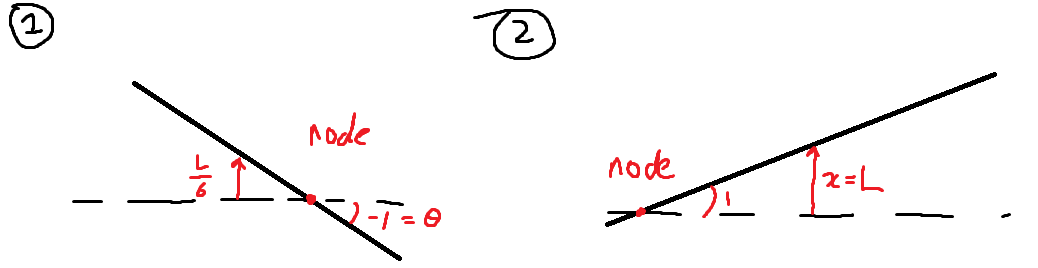
\includegraphics[width=0.5\textwidth]{Questions/Figures/Q4 Mode and Nodes.png}
    \caption{Mode shapes and nodes.}
    \label{fig:Q4 Mode and Nodes}
\end{figure}

